\chapter{Outils et méthodes}
\label{chap:automateVerifOutils}

chapitre sur les outils + moyens pour détecter \medbreak

intro

\section{Modélisation d'une attaque}

En sécurité informatique, la première étape, essentielle avant de développer une solution, c'est de produire un modèle du danger que l'on souhaite cibler. On parle parfois de \textit{modèle de fuite}. Cette étape de synthèse et d'abstraction est importante pour identifer les risques encourus par le futur système, souvent en identifiant les point de fuites employés par les attaques déjà publiées. \citeauthor{BewarCTSideChannel} \cite{BewarCTSideChannel} nous donne les trois modèles d'adversaires que l'on doit considérer lorsque l'on souhaite se défendre contre les attaques temporelles :

\begin{table}[!ht]
  \caption{Modèles d'adversaires pour les attaques temporelles \cite{BewarCTSideChannel}}
  \label{tab:temporal_attacks}
  \begin{adjustbox}{width=\textwidth}
  \begin{tabularx}{\textwidth}{|L|L|}
    \hline
    \rowcolor{lightgray}
    \multicolumn{1}{|C|}{\textbf{Type d'attaque}} & \multicolumn{1}{C|}{\textbf{Description}} \\ \hline
    Par chronométrage & Observation du temps de calcul. \\ \hline
    Par accès mémoire & Manipulation et observation des états d'un ou des caches mémoires. \\ \hline
    Par récupération de traces & Suivi des appels de fonctions, des accès réussis ou manqués à la mémoire. \\ \hline
  \end{tabularx}
  \end{adjustbox}
\end{table}

Ces types d'attaques forment une base pour la conception de nos mdodèles d'attaquant. Considérer le mode opératoire <<récupération de traces>> induit un modèle plus fort. Des travaux comme ceux de \citeauthor{twartingCT} \cite{twartingCT} portent directement sur des améliorations matériel permettant une défense contre ce modèle. Considérer un attaquant plus puissant, avec des accès à des ressources supplémentaires, potentiellement hyptotétique, permet de concevoir un système plus sûr. Certains outils comme \cite{ctfuzz,DATA2} ou cette étude \cite{notThatHardCT} exploitent notamment cette mécanique pour attester de la sécurité d'un programme.\medbreak


Puis, avec ces modèles et les contre-mesures connus, on peut constituer un ensemble de règles qui valident ces risques. \cite{CTsaferCrypto} résume celles-ci en une liste de trois règles :
\begin{enumerate}
  \item Toute boucle révèle le nombre d'itérations effectuées. 
  \item Tout accès mémoire révèle l'adresse (ou l'indice) accédé.
  \item Toute instruction conditionnelle révèle quelle branche a été prise.
\end{enumerate}

Avec ces règles, il est alors possible de créer un outil qui analyse les programmes à sécuriser. C'est de cette façon que le premier outil existant a été produit : \texttt{ctgrind} (2010).\medbreak

D'autres chercheurs comme \citeauthor{binsecRel2019} \cite{binsecRel2019} s'attellent à la création de modèles formels. Cette méthode demande un travail de formalisation du comportement de programmes binaire et une implémentation plus rigoureuse de leurs outils. Cela permet en retour une évaluation complète et correct de programmes complexes (\ie primitives cryptographiques asymétriques).

\subsection*{Formalisation de modèle}

Si on regarde plus en détails les travaux nécessaires à la conception d'un tel modèle, on peut s'appuyer sur l'article \citetitle{formalConstantTime} \cite{formalConstantTime}.\medbreak


On commence par définir un programme. Il s'agit d'une suite d'instruction binaire. Et une instruction est une action sur la mémoire. Cela nous permet de définir notre programme comme une suite de configuration $(l,r,m)$; $l$ la ligne d'instruction, $r$ le dictionnaire de registre et $m$ la mémoire. La configuration initiale est défini par $c_0 \triangleq (l_0,r_0,m_0)$ où $l_0$ est l'adresse de l'instruction d'entrée du programme, $r_0$ un dictionnaire de registre vide et $m_0$ une mémoire vide.\smallbreak

Ainsi, avec cette modélisation, une instruction est un changement appliqué à notre configuration. Ce changement peut être représenté par $ c_0 \underset{f}{\to} c_1 $, $c_0$ et $c_1$ deuc configurations successives, $\to$ la transition entre les deux et $f$ une fuite émise par cette transition. Notons que certaines instructions ne produisent pas de fuites.\smallbreak

Une fois ce préambule installé on peut alors définir formellement le comportement d'une instruction. Si on regarde par exemple 

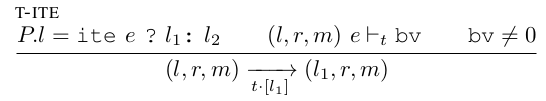
\includegraphics{pictures/branchement.png}
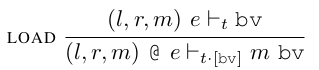
\includegraphics{pictures/load.png}
\newpage



- formalisation des regles de securite


The behavior of the program is modeled
with an instrumented operational semantics taken from [69]
in which each transition is labeled with an explicit notion of
leakage. A transition from a configuration c to a configuration
c0 produces a leakage t, denoted c → c0 . Analogously, the
t
evaluation of an expression e in a configuration (l, r, m),
denoted (l, r, m) e `t bv, produces a leakage t. The leakage
of a multistep execution is the concatenation of leakages
produced by individual steps. We use → k with k a natural
t
number to denote k steps in the concrete semantics.
An excerpt of the concrete semantics is given in Fig. 3
where leakage by memory accesses occur during execution of
load and store instructions and control flow leakages during
execution of dynamic jumps and conditionals. The full set of
rules is given in Appendix A1.



\cite{binsecRel2019}


\section{Analyse d'un programme}


4.1
Static analysis
Static analysis approaches attempt to derive security properties
from the program without actually executing it, extracting formally
defined guarantees on all possible executions through binary or
source code analysis. As a formal exploration of every reachable
state is unfeasible, program behavior is often approximated, making
them prone to false positives. Static approaches were the first to be
considered, as side-channel security is closely related to information
flow policies [53].
4.1.1 Logical reduction Non-interference is a 2-safety property stat-
ing that two executions with equivalent public inputs and poten-
tially different secret inputs must result in equivalent public outputs.
This definition covers side channels by considering resource usage
(e.g., address trace) as a public output. Approaches based on logical
reduction to 1-safety transform the program so that verifying its
side-channel security amounts to proving the safety of the trans-
formed program.
Self-composition [23] interleaves two executions of a program P
with different sets of secret variables in a single self-composed pro-
gram P;P' . Solvers can then be used to verify the non-interference
property. This approach was used by Bacelar Almeida et al. [15]
to manually verify limited examples, relying on a large amount of
code annotations. ct-verif instead runs the two copies in lockstep,
while checking their assertion-safety [13]. It is able to verify LLVM
programs, leveraging the boogie verifier. Sidetrail [19] reuses this
to verify that secret dependent branches are balanced (assuming
a fixed instruction cost and excluding memory access patterns),
providing a counter-example when this verification fails.
However, such approaches suffer from an explosion in the size of
the program state space. Blazer [17] verifies timing-channel security
on Java programs by instead decomposing the execution space into
a partition on secret-independent branches. Proving 2-safety is
thus reduced to verifying 1-safety on each trace in the partition
improving scalability at the cost of precision. Themis [48] uses static
taint analysis to automatically annotate secret-dependent Java code
with Hoare logic formulas as pre- and post-conditions. An SMT
solver then verifies that the post-condition implies execution time
differences remain bounded by given constant. Both tools provide
a witness triggering the vulnerability otherwise.
4.1.2 Type systems Approaches based on verifying type safety of
a program differ from language-level countermeasures [12, 30], as
CCS ’23, November 26–30, 2023, Copenhagen, Denmark
the developer only needs to type the secret values with annotations
instead of rewriting the program. The type system then propagates
this throughout the program, similarly to static taint analysis. Type
systems were considered relatively early to verify non-interference
properties [7] and offer good scalability but their imprecision makes
them difficult to use in practice.
VirtualCert [22] analyzes a modified CompCert IR where each
instruction makes its successors explicit. The authors define seman-
tics for that representation, building the type system on top of it.
An alias analysis giving a sound over-approximated prediction of
targeted memory address is needed to handle pointer arithmetic.
While this approach is more suited to a strict verification task, it
can also provide a leakage estimate.
FlowTracker [107] introduces a novel algorithm to efficiently
compute implicit information flows in a program, and uses it to
apply a type system verifying constant-time.
4.1.3 Abstract interpretation As a program semantics is generally
too complex to formally verify non-trivial properties, abstract in-
terpretation [50] over-approximates its set of reachable states, so
that if the approximation is safe, then the program is safe.
CacheAudit [55] performs a binary-level analysis, quantifying
the amount of leakage depending on the cache policy by finding
the size of the range of a side-channel function. This side-channel
function is computed through abstract interpretation, and the size
of its range determined using counting techniques. It was later
extended to support dynamic memory and threat models allowing
byte-level observations [56] and more x86 instructions [91].
Blazy et al. [28] focus on the source code instead of the binary.
Their tool is integrated into the formally-verified Verasco static an-
alyzer, and uses the CompCert compiler. The analysis is structured
around a tainting semantics that propagates secret information
throughout the program.
STAnalyzer [110] uses data-flow analysis to report secret-dependent
branches and memory accesses.
CacheS [126] uses an hybrid approach between abstract interpre-
tation and symbolic execution. The abstract domain keeps track of
program secrets—with a precise symbolic representation for values
in order to confirm leakage—but keeps only a coarse-grain rep-
resentation of non-secret values. To improve scalability, CacheS
implements a lightweight but unsound memory model.
4.1.4 Symbolic execution Symbolic execution [81] (SE) denotes
approaches that verify properties of a program by executing it with
symbolic inputs instead of concrete ones. Explored execution paths
are associated with a logical formula: the conjunction of condi-
tionals leading to that path. A memory model maps encountered
variables onto symbolic expressions derived from the symbolic in-
puts and the concrete constants. A solver is then used to check
whether a set of concrete values satisfies the generated formulas.
Recent advances in SMT solvers have made symbolic execution a
practical tool for program analysis [42].
CoCo-Channel [34] identifies secret-dependent conditions us-
ing taint-analysis, constructs symbolic cost expressions for each
path of the program uses SE and reports paths that exhibit secret-
dependent timing behavior. Their cost model assigns a fixed cost
per instruction, excluding secret-dependent memory accesses.CCS ’23, November 26–30, 2023, Copenhagen, Denmark
Several works use symbolic execution to derive a symbolic cache
model and check that cache behavior does not depend on secrets.
CANAL [117] models cache behaviors of programs directly in the
LLVM intermediate representation by inserting auxiliary variable
and instructions. It then uses KLEE [41] to analyze the program
and check that the number of hits does not depend on secrets.
Similarly, CacheFix [47] uses SE to derive a symbolic cache model
supporting multiple cache policies. In case of a violation, CacheFix
can synthesize a fix by injecting cache hits/misses in the program.
CaSym [35] follows the same methodology and, to improve scala-
bility, includes simplifications of the symbolic state and loop trans-
formations, which are sound but might introduce false positives.
SE suffers from scalability issues when applied to 2-safety prop-
erties like constant-time verification. Daniel et al. [51] adapt its
formalism to binary analysis, introducing optimizations to maxi-
mize information shared between two executions following a same
path. Their framework Binsec/Rel offers a binary-level CT analysis,
performing a bounded exploration of reachable states and giving
counterexamples for the identified vulnerabilities.
Pitchfork [54] combines SE and dynamic taint tracking. It soundly
propagates secret taints along all executions paths, reporting tainted
branch conditions or memory addresses. Interestingly, Pitchfork
can analyze protocol-level code by abstracting away primitives’ im-
plementations using function hooks, and analyzing them separately.
ENCIDER [140] combines symbolic execution with taint analysis
to reduce the number of solver calls. It also enables to specify
information-flow function summaries to reduce path explosion.
4.2
Dynamic analysis
Dynamic analysis groups approaches that derive security guar-
antees from execution traces of a target program. Some form of
dynamic binary instrumentation (DBI) is often used to execute the
program and gather events of interest, such as memory accesses or
jumps. Dynamic approaches differ in the events collected, and how
traces are processed. They can be grouped depending on whether
they reason on a single trace, or compare multiples traces together.
4.2.1
Trace comparison approaches
Statistical tests. Statistical tests can be used to check if different
secrets induce statistically significant differences in recorded traces.
Cache Template [70] monitors cache activity to detect lines associ-
ated with a target event, then finds lines correlated with the event
using a similarity measure. A first pass using page-level observa-
tions instead of lines can be used to improve scalability [112]. Shin
et al. [114] use K-means clustering to produce two groups of traces
for each line. The confidence in the partition indicates which line
is likely to be secret-dependent. DATA [132] employs a Kuiper test
then a Randomized Dependence Coefficient test to infer linear and
non-linear relationships between traces and secrets. This was later
extended to support cryptographic nonces as secrets [130].
Mutual information (MI) can be used to quantify the information
shared between secret values and recorded traces, with a non-zero
MI score giving a leakage estimation. MicroWalk [133] computes
MI scores between input sets and hashed traces, with leakage lo-
cation pinpointed using finer-grained instruction-level MI scores.
MicroWalk-CI [134] optimizes this process by transforming the
Geimer et al.
traces in call trees, and adds support for JavaScript and easy inte-
gration in CI, following recommendations from [73]. CacheQL [141]
reformulates MI into conditional probabilities, estimated with neu-
ral networks. Leakage location is estimated by recasting the problem
into a cooperative game solved using Shapley values. Contrary to
other tools [20, 133], CacheQL does not assume uniform distribu-
tion of the secret, nor deterministic executions traces.
STACCO [136] targets control-flow vulnerabilities specifically in
TLS libraries running on SGX, focusing on oracles attacks [11, 29].
Traces recorded under different TLS packets are represented as
sequences of basic blocks and compared using a diff tool.
Instead of recording traces, dudect [106] records overall clock
cycles and compares their distribution with secret inputs divided
in two classes (fix-vs-random). While this approach is simple and
lightweight, it gives certainty that an implementation is secure up
to a number of measurements. Contrary to other tools relying on
an explicit leakage model, dudect directly monitors timings. Hence,
vulnerabilities to other microarchitectural attacks like Hertzbleed
might (in theory) be detected by dudect.
Fuzzing. Fuzzing techniques can be used to find inputs maximiz-
ing coverage and side-channel leakage. DifFuzz [95] combines
fuzzing with self-composition to find side-channels based on in-
struction count, memory usage and response size in Java programs.
ct-fuzz [72] extends this method to binary executables and cache
leakage.
4.2.2 Single trace Other approaches use only one trace to perform
the analysis, sacrificing coverage for scalability. ctgrind [85] re-
purposes the dynamic taint analysis of Valgrind to check CT by
declaring secrets as undefined memory. This solution is easy to
deploy and reuses familiar tools, but remains imprecise.
ABSynthe [66] identifies secret-dependent branches using dy-
namic taint analysis. It employs a genetic algorithm to build a
sequence of instructions based on interference maps evaluating
contention created by each x86 instructions.
More precise approaches use SE to replay the trace with the
secret as a symbolic value and check for CT violation. CacheD [127]
applies this approach to memory accesses. Abacus [20] extends it
to control-flow vulnerabilities, picking random values to check
satisfiability instead of using a SMT solver. It also includes leakage
estimation through Monte Carlo simulation.
Finally, CaType [74] uses refinement types (i.e., types carrying
a predicate restricting their possible values) on a trace to track
constant bit values and improve precision. CaType also supports
implementations that use blinding.



\raggedbottom
\textit{Transition}

